\section{幂函数、指数函数、对数函数}
\begin{definition}
同一个数\(a\ (a\in\mathbb{R})\)连续相乘\(b\ (b\in\mathbb{N})\)次所得的乘积,
称作“\(a\)的\(b\)次方”
或“\(a\)的\(b\)次幂”,
记作\(a^b\),
即\[
	a^b
	\defeq
	\underbrace{a \times a \times \dotsm \times a}_{\text{$b$次}} = \prod_{i=1}^b a.
\]

特别地,规定:\begin{gather*}
	a^0 \defeq 1 \quad(a\neq0), \\
	a^{-1} \defeq \frac1a \quad(a\neq0), \\
	a^{-n} \defeq \frac1{a^n} \quad(a\neq0), \\
	a^{1/n} \defeq \sqrt[n]{a} \quad(a\geq0). \\
\end{gather*}
\end{definition}

\begin{figure}[htb]
	\centering
	\begin{tikzpicture}
		\def\r{\textcolor{orange}}
		\def\b{\textcolor{blue}}
		\def\p{\textcolor{purple}}
		\draw(0,0)node{\(\r{a}^{\b{b}} = \p{c} \defiff \log_{\r{a}} \p{c} = \b{b}\)};
		\draw(-2.2,-.5)node{\r{底数}}
			(-2.2,.5)node{\b{指数}}
			(-1,-.5)node{\p{幂}}
			(.3,-.5)node{\r{底数}}
			(1.4,-.5)node{\p{真数}}
			(2.3,.5)node{\b{对数}};
		\draw[->](-1.7,-.3)--(-1.7,-1)--(.84,-1)->(.84,-.3); %a
		\draw[->](-1.55,.3)--(-1.55,1)--(1.7,1)->(1.7,.3); %b
		\draw[->](-.86,.3)--(-.86,.7)--(1.1,.7)->(1.1,.3); %c
	\end{tikzpicture}
	\caption{底数、指数、幂与对数的联系}\label{figure:函数.底数、指数、幂与对数的联系}
\end{figure}

\begin{proposition}
\(1\)的任意次幂还是\(1\),即\(1^n = 1\).
\end{proposition}

\begin{proposition}
\(0\)的任意非零次幂还是\(0\),即\(0^n = 0\ (n\neq0)\).
\end{proposition}

\subsection{幂函数的概念}
\begin{definition}[幂函数]
函数\(f(x)=x^{\mu}\ (\mu \in \mathbb{R})\),
称为\DefineConcept{幂函数}.
\end{definition}

\subsection{幂函数的性质}
\begin{property}
幂函数具有以下性质:
\begin{itemize}
	\item 当\(\mu = 0\)时,
	幂函数\(f(x)=x^{\mu}\)在定义域\((-\infty,+\infty)\)上恒为一,
	是常数函数.

	\item 当\(\mu\)为正奇数时,
	幂函数\(f(x)=x^{\mu}\)为奇函数,
	其定义域、值域均为\((-\infty,+\infty)\),它在定义域内恒单调递增.

	\item 当\(\mu\)为正偶数时,
	幂函数\(f(x)=x^{\mu}\)为偶函数,
	其定义域为\((-\infty,+\infty)\),其值域为\([0,+\infty)\),
	它在\((-\infty,0]\)上单调递减,在\([0,+\infty)\)上单调递增.

	\item 当\(\mu\)为负奇数时,
	幂级数\(y=x^{\mu}\)又称为\DefineConcept{比例函数},
	其定义域、值域为\((-\infty,0)\cup(0,+\infty)\),
	它在区间\((-\infty,0)\)和\((0,+\infty)\)内单调递减.

	若幂函数前有常系数大于零则称之为\DefineConcept{正比例函数}.
	%@Mathematica: Plot[Evaluate[x^-n /. n -> {1, 2, 3, 4, 5}], {x, 0, 2}, PlotRange -> {0, 2}, PlotLegends -> Automatic]

	若幂函数前有常系数小于零则称之为\DefineConcept{反比例函数}.
	%@Mathematica: Plot[Evaluate[x^-n /. n -> {1, 2, 3, 4, 5}], {x, -2, 0}, PlotRange -> {-2, 2}, PlotLegends -> Automatic]

	\item 当\(\mu\)为负偶数时,
	幂函数\(f(x)=x^{\mu}\)为偶函数,
	其定义域为\((-\infty,0)\cup(0,+\infty)\),其值域为\((0,+\infty)\),
	它在\((-\infty,0)\)内单调递增,在\((0,+\infty)\)内单调递减.

	\item 当\(\mu = \pm\frac{m}{n} \in \mathbb{Q}\)(\(m,n>0\)且\(m\)、\(n\)是互素的整数)时,
	幂函数\(f(x)=x^{\mu}=x^{\pm\frac{m}{n}}\)可改写为\(y=\sqrt[n]{x^m}\)(\(\mu>0\)时)
	或\(y=\frac{1}{\sqrt[n]{x^m}}\)(\(\mu<0\)时).
\end{itemize}
\end{property}

\begin{figure}[htb]
	\centering
	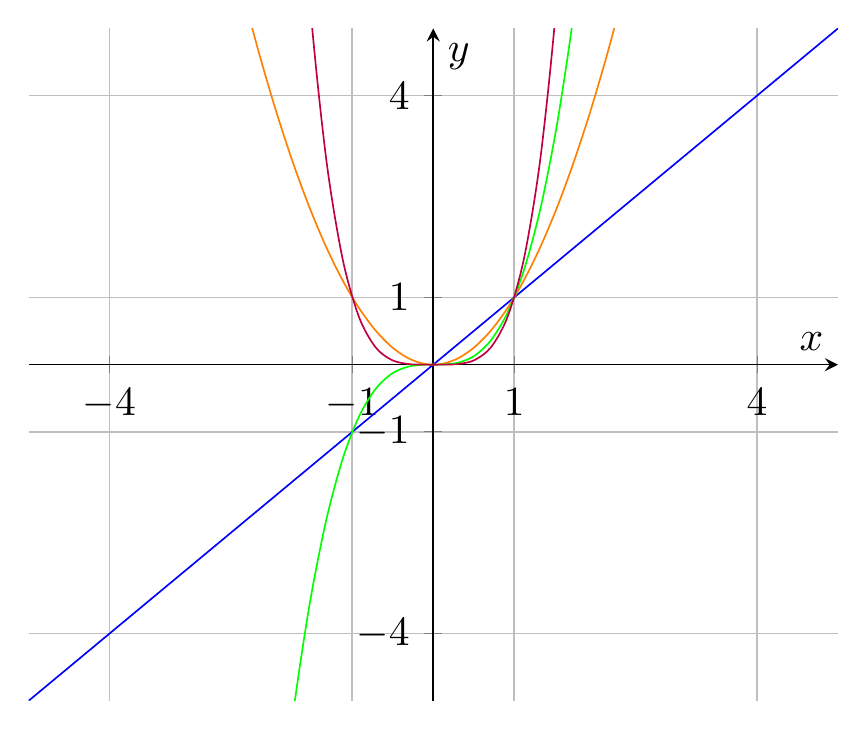
\begin{tikzpicture}[scale=1.5]
		\begin{axis}[
			xmin=-5,xmax=5,
			ymin=-5,ymax=5,
			enlargelimits,
			axis lines=middle,
			xlabel=$x$,
			ylabel=$y$,
			xtick={-4,-1,1,4},
			ytick={-4,-1,1,4},
			grid=major,
		]
			\begin{scope}[samples=50,smooth,domain=-5:5]
				\addplot[color=blue]{x};
				\addplot[color=orange]{x^2};
				\addplot[color=green]{x^3};
				\addplot[color=purple]{x^4};
			\end{scope}
		\end{axis}
	\end{tikzpicture}
	\caption{}
\end{figure}

\begin{figure}
	\centering
	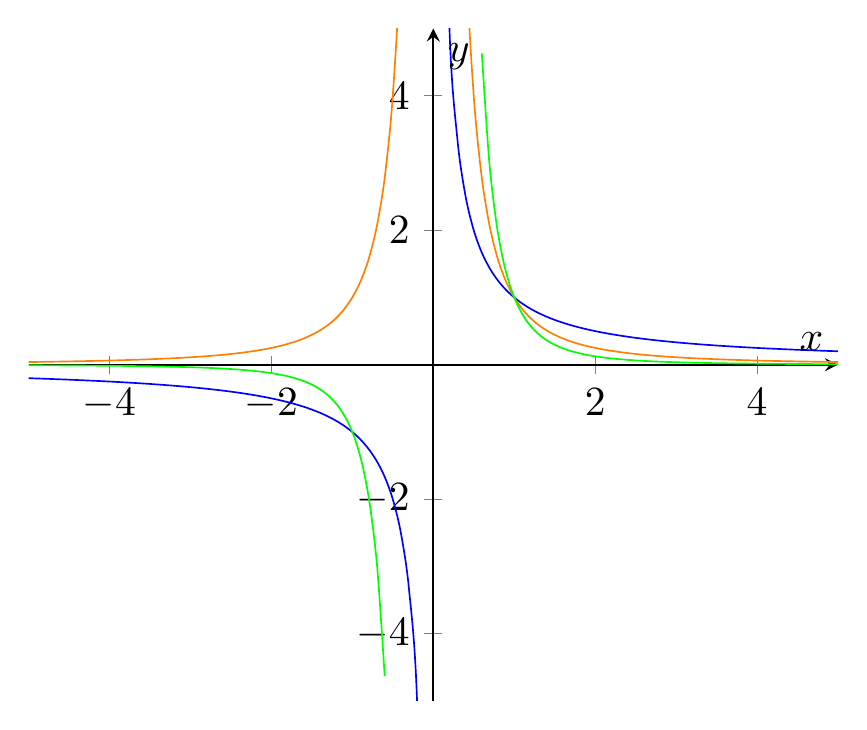
\begin{tikzpicture}[scale=1.5]
		\begin{axis}[
			xmin=-5,xmax=5,
			ymin=-5,ymax=5,
			enlargelimits,
			axis lines=middle,
			xlabel=$x$,
			ylabel=$y$,
		]
			\begin{scope}[samples=50,smooth]
				\begin{scope}[domain=-5:-.1]
					\addplot[color=blue]{1/x};
					\addplot[color=orange]{1/(x^2)};
					\addplot[color=green,domain=-5:-.6]{1/(x^3)};
				\end{scope}
				\begin{scope}[domain=.1:5]
					\addplot[color=blue]{1/x};
					\addplot[color=orange]{1/(x^2)};
					\addplot[color=green,domain=.6:5]{1/(x^3)};
				\end{scope}
			\end{scope}
		\end{axis}
	\end{tikzpicture}
	\caption{}
\end{figure}

\subsection{指数函数的概念}
\begin{definition}
设\(a>0\)且\(a \neq 1\).
把函数\(f(x)=a^x\)
称为“以\(a\)为底的\DefineConcept{指数函数}”.
\end{definition}

\begin{theorem}
设\(f\)是以\(a\)为底的指数函数,
则\(f\)存在反函数.
\begin{proof}
指数函数是单调函数.
\end{proof}
\end{theorem}

\subsection{指数函数的性质}
\begin{property}
\begin{gather}
	a^x a^y = a^{x+y}, \\
	\frac{a^x}{a^y} = a^{x-y}, \\
	(a^x)^y = a^{xy}.
\end{gather}
\end{property}

\subsection{对数函数的概念}
\begin{definition}
设\(a>0\)且\(a\neq1\).
以\(a\)为底的指数函数的反函数,
称为“以\(a\)为底的\DefineConcept{对数函数}”,
记作\(\log_a x\),
即\begin{equation}\label{equation:函数.对数的定义}
	y = \log_a x
	\defiff
	a^y = x.
\end{equation}
%@see: https://mathworld.wolfram.com/Logarithm.html
\end{definition}

以\(10\)为底的对数,称为\DefineConcept{常用对数},记作\(y = \lg x\),
即\begin{equation}
	\lg x \defeq \log_{10} x.
\end{equation}

以常数\(e\)为底的对数,称为\DefineConcept{自然对数},记作\(y = \ln x\),
即\begin{equation}
	\ln x \defeq \log_e x.
\end{equation}

\subsection{对数函数的性质}
\begin{proposition}[对数恒等式]
设\(a>0,a\neq1\),
则对\(\forall x>0\)
有\begin{equation}\label{equation:函数.对数恒等式}
	a^{\log_a x} = x.
\end{equation}
\begin{proof}
根据\hyperref[equation:函数.对数的定义]{对数的定义}有
\(y = \log_a x
\defiff
a^y = x\),
于是\(a^{\log_a x} = a^y = x\).
\end{proof}
\end{proposition}

\begin{theorem}
设\(a>0,a\neq1\),
则\begin{gather}
	\log_a 1 = 0, \\
	\log_a a = 1.
\end{gather}
\end{theorem}

\begin{theorem}[对数的运算法则]
设\(a>0,a\neq1,x>0,y>0\),
则\begin{gather}
	\log_a xy = \log_a x + \log_a y,
		\label{equation:函数.对数的基本运算法则1} \\
	\log_a \frac{x}{y} = \log_a x - \log_a y,
		\label{equation:函数.对数的基本运算法则2} \\
	\log_a x^y = y \log_a x.
		\label{equation:函数.对数的基本运算法则3}
\end{gather}
\end{theorem}

\begin{theorem}[换底公式]
设\(a>0,a\neq1,c>0,c\neq1,b>0\),
则\begin{equation}\label{equation:函数.换底公式}
	\log_a b = \frac{\log_c b}{\log_c a}.
\end{equation}
\begin{proof}
由\hyperref[equation:函数.对数恒等式]{对数恒等式}有\(b = a^{\log_a b}\),
于是\(\log_c b
= \log_c a^{\log_a b}\).
又由有\hyperref[equation:函数.对数的基本运算法则3]{对数的运算法则}有\[
	\log_c a^{\log_a b} = \log_a b \cdot \log_c a,
\]
所以\(\log_a b = \frac{\log_c b}{\log_c a}\).
\end{proof}
\end{theorem}

\begin{corollary}
设\(a>0,a\neq1,b>0,b\neq1\),
则\begin{equation}
	\log_a b = \frac1{\log_b a}.
\end{equation}
\begin{proof}
在\hyperref[equation:函数.换底公式]{换底公式}中,令\(c=b\)便得.
\end{proof}
\end{corollary}

\begin{corollary}
设\(a>0,a\neq1,a^x\neq1\)
则\begin{equation}
	\log_{a^x} b^y = \frac{y}{x} \log_a b.
\end{equation}
\end{corollary}

\begin{example}
设\(a>0,b>0\).
证明:\begin{equation}\label{equation:函数.真底互换公式}
	a^{\ln b} = b^{\ln a}.
\end{equation}
\begin{proof}
在\cref{equation:函数.真底互换公式} 等号左右变量分别取对数,
得\[
	\ln(a^{\ln b}) = \ln b \ln a, \qquad
	\ln(b^{\ln a}) = \ln a \ln b,
\]
显然两者相等,故\(a^{\ln b} = b^{\ln a}\)成立.
\end{proof}
\end{example}

\subsection{重幂}
设\(a\)是实数,\(b\)是正整数.
定义:\[
	\relax^ba \defeq \underbrace{a^{a^{\iddots^a}}}_{\text{\(b\)个}},
\]
我们把\(\relax^ba\)读作“\(a\)的\(b\)~\DefineConcept{重幂}”.

例如,\[
	\relax^23 = 3^3, \qquad
	\relax^33 = 3^{3^3}, \qquad
	\relax^43 = 3^{3^{3^3}}.
\]
